
\documentclass[a4paper,12pt,oneside]{report}
\usepackage{OvidiusFMI}

\usepackage{times}
\usepackage[T1]{fontenc}
\usepackage[utf8]{inputenc}
\usepackage{graphicx}
\usepackage{hyperref}
\usepackage{color,xcolor}
\usepackage{framed}
\usepackage{enumerate}
\usepackage{listings}
\usepackage{amsmath,amsfonts,amssymb,amsthm,epsfig,epstopdf,url,array}
\usepackage{tikz-cd}
\usepackage{multicol,multirow}
\usepackage{enumitem}

\include{custom-lst-style}

\setlength{\parindent}{0pt}
\setlength{\parskip}{1\baselineskip}

\facultatea{Matematică și Informatică}
\specializarea{Informatică}
\teza{licență}
\titlu{PresSync — Sistem Autonom de Gestiune a Prezenței \\ bazat pe Conectivitate Wi-Fi la Nivelul Stratului 2}
\gradDidacticCP{Conf. univ. dr.}
\coordonatorPrincipal{Constantin-Claudiu Gava}
\autor{Moraru Vlad}
\data{2026}

\begin{document}
\maketitle

\pagenumbering{roman}
\tableofcontents
\listoffigures
\newpage
\pagenumbering{arabic}

\chapter{Introducere}

Prezenței participanților la activități educaționale, profesionale sau organizaționale este o provocare în contextul actual. Metodele actuale de pontaj — apelul nominal, listele pe hârtie sau cartelele de acces fizice — sunt lente, predispuse la erori și vulnerabile, precum înregistrarea prezenței în locul unui coleg absent. Soluțiile digitale existente, bazate pe coduri QR, localizare GPS sau platforme cloud, adresează parțial aceste neajunsuri, însă introduc alte limitări: dependența de conexiunea la internet, riscul falsificării locației sau preocupări legate de confidențialitatea datelor personale.

Lucrarea mea propune ca solutie  PresSync — un sistem autonom de gestionare a prezenței, care utilizează infrastructura Wi-Fi locală ca mecanism de validare a prezenței fizice.

\section{Structura lucrării}

Lucrarea este structurată în cinci capitole, organizate progresiv de la analiza problemei până la implementarea și evaluarea soluției propuse.

\begin{itemize}
    \item \textbf{Capitolul 1 — Introducere} oferă o imagine de ansamblu asupra contextului care a motivat dezvoltarea sistemului PresSync, prezintă pe scurt soluția propusă și descrie structura lucrării.
    \item \textbf{Capitolul 2 — Definirea problemei} analizează metodele actuale de pontaj și limitările acestora, realizează o comparație structurată a soluțiilor existente pe piață și fundamentează arhitectural alegerea abordării bazate pe conectivitate Wi-Fi la nivelul Stratului 2.De asemenea ,capitolul defineste obiectivele sistemului, actorii implicați și scenariile de bază de utilizare.
    \item \textbf{Capitolul 3 — Analiza software} prezintă cerințele funcționale și non-funcționale ale aplicației, modelul funcțional al sistemului, descrierea detaliată a cazurilor de utilizare și diagramele UML asociate.
    \item \textbf{Capitolul 4 — Proiectare și implementare} descrie arhitectura tehnică a soluției, incluzând proiectarea bazei de date, tehnologiile utilizate, diagramele de interacțiune și de clase, precum și secvențe reprezentative de cod sursă.
    \item \textbf{Capitolul 5 — Concluzii} sintetizează contribuțiile proprii aduse prin această lucrare, evaluează rezultatele obținute în raport cu obiectivele definite și propune direcții de dezvoltare ulterioară a sistemului.
\end{itemize}
\newpage
\chapter{Definirea problemei}
    Acest capitol definește problema gestionării prezenței în diferite contexte și oferă o imagine de ansamblu asupra sistemelor actuale de pontaj și a limitărilor acestora. De asemenea, este realizată o analiză comparativă a modelelor existente cu soluția propusă de mine și se enumeră obiectivele acesteia. Capitolul se încheie cu definirea actorilor și sistemului și prezentarea scenariilor de bază de utilizare. 
\section{Introducere și Contextualizare}
Dacă ai participat vreodată la un curs, o ședință sau o conferință, știi că momentul în care se face prezența este o pierdere de timp. Listele pe hârtie circulate prin sală, strigarea fiecărui nume sau distribuirea cartelelor de acces sunt soluții banale, dar ele ascund probleme reale: timp pierdut, erori frecvente și participanți care sunt pe listă deși nu se află în cameră.

Această situație, unde un coleg îl marchează pe altul prezent deși nu e adevărat, nu este doar o nedreptate față de ceilalți, dar creează și o greșeală în datele colectate. Acest lucru poate afecta decizii ce țin de evaluare sau de monitorizarea activității. Această problemă nu este una trivială, deoarece, cu cât grupul este mai mare cu atât crește riscul ca astfel de situații să treaca neobservate.

Este important să evidențiem că această problemă nu aparține doar mediului universitar, chiar dacă soluția mea a pornit de acolo. Ea poate fi aplicată și în medii cum ar fi o conferință sau orice alt tip de eveniment unde organizatorul ar avea nevoie să știe exact numărul de participanți și cine sunt ei, pentru a crea mai apoi statistici sau rapoarte pentru planificarea următorului eveniment. Deci, cum verificăm că oamenii sunt cu adevărat acolo, fără a întrerupe activitatea și fără a permite date inexacte? Avem nevoie de un mecanism de înregistrare a prezenței care să fie fiabil, rapid și capabil să genereze informațiile utile, nu o simplă listă bifată în grabă

\noindent\rule{\textwidth}{0.4pt}

\section{Analiza soluțiilor existente}

Pe piață există deja o varietate largă de soluții care gestionează prezența. De la liste de hârtie, carduri fizice până la platforme cloud sofisticate.
Problema nu este lipsa soluțiilor, ci faptul că multe din ele nu rezolvă în totalitate problema.

Unele sisteme necesită costuri suplimentare pentru a fi implementate. Echipamente hardware dedicate și o infrastructură tehnică.
Alte soluții sunt mai accesibile dar nu oferă garanția că persoana se află fizic în încăpere.

În toate mediile, nevoia principală rămâne aceeași: o soluție ușor de folosit, de implementat și care nu permite fraudă. Acest echilibru este ceea ce lipsește majorității soluțiilor.
Pentru a înțelege exact unde se situează PresSync, urmează să prezint o comparație cu cele trei tipuri de sisteme care sunt cel mai des utilizate în prezent.
\subsection{Sistemele cu cartele magnetice}

Cartelele magnetice sunt probabil cele mai cunoscute soluții de control al accesului pe care le putem întâlni. Funcționarea lor se bazează pe principiul că participantul deține un obiect fizic, pe care îl prezintă unui cititor la intrarea în spațiu. Prezența și autentificarea au loc instant. Simplitatea este punctul forte al acestui tip de soluții: scanarea rapidă, infrastructura conectată prin cablu la serverele instituției și funcționează într-o rețea izolată.

Problema principală o constituie costurile care sunt semnificative: cumpărarea și instalarea cititoarelor la fiecare intrare, mentenanța continuă și înlocuirea periodică a cartelelor pierdute sau deteriorate. De asemenea, sistemul este ancorat de acea zonă. Mai mult de atât există și riscul ca un coleg să îi dea cartela altuia pentru a fi marcat prezent.

\subsection{Sisteme mobile bazate pe scanare de coduri QR}
Codul QR afișat pe un videoproiector a devenit ceva familiar în sălile de curs în ultimii ani. Se generează un cod QR, care mai apoi este proiectat, iar studenții scanează codul cu telefonul.
Implementarea nu necesită hardware suplimentar, sistemul se folosește de tehnologia existentă deja și poate fi pus în funcțiune în câteva minute.

Această abordare este una ideală în contextul educațional unde bugetul este limitat. Însă problema acestei soluții este securitatea, deoarece ea se bazează pe faptul că doar persoanele prezențe fizic au acces la cod, însă această ipoteză nu poate fi adevărată. Un singur participant din sală poate fotografia codul și îl trimite pe WhatsApp oricui. Nici versiunile cu coduri dinamice nu rezolvă complet problema: codul poate fi partajat în timp real.
\subsection{Sisteme de tracking pe bază de localizare GPS}
Aceste platforme au o abordare diferită. Ele verifică dacă participantul se află în locul potrivit. Utilizatorul are nevoie doar să facă un check-în din aplicație, iar sistemul compară coordonatele GPS ale telefonului cu o zonă predefinită în aplicație.

Această soluție este flexibilă, nu are nevoie de o infrastructură hardware, evenimentul poate fi configurat oriunde. Totuși pentru săli de curs, birouri etc., această abordare are trei probleme.

Prima este falsificarea coordonatelor GPS. Există aplicații specializate care permit simularea unei locații. A două problemă este confidențialitatea. Și a treia limitare este de natură tehnică, sistemul are nevoie de o conexiune constantă la internet. În spații cu semnal slab aplicația devine inoperabilă.
\newpage
\subsection{Sinteza comparativa}

\begin{table}[htbp]
    \centering
    \small
    \setlength{\tabcolsep}{3pt}
    \begin{tabular}{|p{0.17\textwidth}|p{0.18\textwidth}|p{0.18\textwidth}|p{0.18\textwidth}|p{0.18\textwidth}|}
        \hline
        \textbf{Criteriu comparativ} & \textbf{Sisteme RFID / Cartele} & \textbf{Scanare Cod QR} & \textbf{Tracking GPS (Cloud)} & \textbf{PresSync} \\
        \hline
        Costuri de implementare & Ridicate (necesită hardware dedicat și cartele) & Foarte scăzute (folosește infrastructura mobilă existentă) & Medii spre ridicate (abonamente SaaS/Cloud) & Scăzute (necesită un router compatibil OpenWRT și/sau un sistem embedded) \\
        \hline
        Risc de fraudă & Ridicat (delegarea fizică a token-ului de autentificare) & Foarte ridicat (redistribuirea codului optic în afara perimetrului) & Ridicat (falsificarea coordonatelor GPS prin location mocking) & Scăzut (conectivitatea la nivelul Stratului 2 este condiționată de atenuarea fizică a semnalului Wi-Fi) \\
        \hline
        Versatilitate & Redusă (infrastructură fixă, instalată permanent) & Ridicată & Foarte ridicată & Ridicată (echipament portabil, instalabil în orice spațiu cu alimentare electrică) \\
        \hline
        Dependență de conexiune externă & Nu (funcționează de regulă în rețea Intranet) & Da & Da (obligatoriu) & Nu (sistemul funcționează într-un mediu de rețea complet izolat, fără conexiune externă) \\
        \hline
    \end{tabular}
    \caption{Comparație între principalele soluții de gestionare a prezenței}
    \label{tab:sinteza-comparativa}
\end{table}

\subsection{Fundamentarea arhitecturală a soluției PresSync}
Analizând comparația, putem să ne dăm seama că fiecare abordare expune o problemă, fie securitatea, fie accesibilitatea economică. PresSync a fost conceput pentru a rezolva toate aceste probleme prin valorificarea proprietății fizice a semnalului Wi-Fi.

Primul pas este înlocuirea cartelei cu dispozitivul mobil personal, ceea ce practic rezolvă împrumutarea token-ului unui coleg. Identitatea digitală a participantului este stocată sub forma unui token JWT, legat de contul său și accesibil exclusiv prin autentificare, ceea ce transformă dispozitivul într-un factor de autentificare.

Elemetul principal al arhitecturii PresSync , și diferență cea mai mare de soluțiile analizate mai sus , este folosirea proprietăților fizice ale undelor radio ca barieră antifraudă.Această abordare este mai robustă ,deoarece validarea prezenței se face prin conectivitate la nivelul Stratului 2 (Data link layer) al modelului OSI. Routerul este configurat în regim de portal captiv , emite pe benzile 2,4GHz și 5GHz, frecvente care sunt sensibile la obstacole fizice din mediul înconjurător.

Atunci când traversează materiale de construcție uzuale , cum ar fi pereți din beton , cărămidă sau gips-carton , semnalul suferă o atenuare destul de mare.
Ceea ce face ca semnalul emis să fie insuficient pentru ca un dispozitiv să se conecteze de la câțiva metri de punctul de acces.Prin urmare , pentru a transmite token-ul JWT și a înregistra prezența , telefonul trebuie să se afle fizic în interiorul spațiului delimitat de router.

Încă un factor care contribuie la această restricție naturală este zona Fresnel. Obstacolele solide intersectate de această zonă reduc puterea semnalului.Combinând acești doi factori , transformăm pereții încăperii într-o barieră naturală antifraudă.

Acest ultim factor previne atacurile de tip MAC spoofing care necesită prezența fizică în raza de acțiune a routerului și echipament specializat.

Încă un factor important al sistemului este independență față de conexiunea la internet . Aplicația rulează local , nu există servere externe , abonament cloud etc.
Această alegere aduce două consecințe practice : Prima este ca sistemul funcționează în orice spațiu cu alimentare electrică.A două este ca datele sunt procesate local fără a fi transmise la alte servicii.

În concluzie PresSync rezolva problema la un nivel mai profund.Ancorând validarea prezenței în proprietăți fizice și eliminând dependență de infrastructura externă.

\section{Descrierea problemei și soluția propusă}


Pe baza secțiunilor prezentate mai sus , putem formula problema principală pe care sistemul o abordează: necesitătea unui mecanism de înregistrare a prezenței care să ofere certitudinea prezenței fizice reale a participantilor, fără prea multe costuri sau dependente de conexiunea externă și păstrarea datelor local.
Având în vedere deficientele solutiilor deja existente mentionate anterior , am considerat necesar construirea unei soluții gazdute local pe un router OpenWRT , în care prezența fizică în retea este dovada participării.Ceea ce elimina dependență de internet sau servicii GPS.PresSync automatizează pontajul , printr-o metoda sigura , rapida și utila.Contextele aplicarii pot fi variate , de la mediul academic până la conferinte și evenimente temporare

\section{Obiectivele sistemului}

Pentru a materializa viziunea descrisa mai sus , am fost ghidat de urmatoare obiective functionale și tehnice:


\begin{enumerate}
[leftmargin=*,label=\textbf{O\arabic*.}]

    \item \textbf{Funcționare autonomă și independență hardware.}
    Sistemul este proiectat să ruleze  \newline izolat pe echipamente accesibile, precum un
    router OpenWRT. Această abordare elimină complet dependența de o conexiune
    la internet sau de servere \textit, asigurând
    un mediu securizat și  în care prezența în rețeaua fizică
   constituie dovada fundamentală a participării.
  

    \item \textbf{Automatizarea calendarului și a recurenței.}
   sistemul preia
    munca repetitivă a admi-nistratorului. Odată definită o categorie de evenimente
    împreună cu regulile sale de recurență (zilnic, săptămânal etc.), aplicația
    instanțiază automat noi evenimente la momentul oportun, fără nicio intervenție
    manuală.

    \item \textbf{Securizarea și delimitarea strictă a accesului.}
    Autentificarea utilizatorilor este realizată prin \textit{token}-uri JWT, asigurând
    un flux clar de autorizare. Fiecare actor are vizibilitate limitată la resursele
    relevante: participantul își confirmă prezența și își verifică istoricul
    personal, în timp ce organizatorul administrează resursele colective și
    accesează datele întregului grup.

    \item \textbf{Procesare concurentă și scalabilitate ridicată.}
    Sistemul separă operațiile de modificare a datelor (comenzi) de cele de citire
     Această separare asigură că cererile de marcare a
    prezenței sunt procesate instantaneu și fără conflicte, iar cererile complexe
    de calcul al statisticilor rulează pe un flux propriu optimizat, fără a bloca
    aplicația.
 

    \item \textbf{Generarea de statistici în timp real.}
    În loc să stocheze datele în formă brută, sistemul le transformă în informații
    utile la cerere. Acesta calculează procentajul de
    prezență la nivel de utilizator sau eveniment și permite extragerea de rapoarte
    detaliate direct din interfață.
  

\end{enumerate}



\section{Actori principali și delimitarea rolurilor}

    Sistemul PresSync lucrează cu două categorii principale de utilizatori, pe care le putem considera \textit{stakeholder}-ii primari și secundari ai platformei.

\textbf{Administratorul (Organizatorul)} reprezintă \textit{stakeholder}-ul primar. El este responsabil de configurarea evenimentelor și a categoriilor acestora, de gestionarea participanților, de stabilirea re-gulilor de recurență (atunci când evenimentele se repetă) și de generarea rapoartelor statistice. Acest rol are acces complet la toate funcționalitățile de administrare ale sistemului.

\textbf{Participantul} este \textit{stakeholder}-ul secundar. El interacționează cu platforma doar pentru a-și marca prezența la evenimentele la care este înscris și pentru a consulta propriul istoric de participare. Accesul său este strict limitat la informațiile și acțiunile care îl privesc direct.

Această separare clară între roluri nu este întâmplătoare. Ea asigură atât o protecție mai bună a datelor, cât și o experiență adaptată nevoilor fiecărui tip de utilizator. Totodată, respectă principiul privilegiului minim (\textit{principle of least privilege}), conform căruia un utilizator ar trebui să aibă doar accesul strict necesar pentru a-și îndeplini atribuțiile.
\section{Scenarii de baza}

Pentru o mai bună înțelegere a sistemului voi explica pe pasi cum are loc procesul de marcare a prezenței , creare evenimente , vizualizare prezențe și administrare utilizatori.

Pentru acest exemplu vom folosi mediul academic.
\begin{itemize}
    \item Profesorul Vlad Moraru , având deja sistemul activ și fiind conectat la retea, deschide o pagina web și este redirectionat de către portalul captiv pe pagina aplicației PresSync.Se înregistrează sau se autentifica dacă are deja cont , fiind moderator/administrator are nevoie de un cod unic care este transmis pe emailul introdus.

    \item După completarea formularului este redirectionat pe pagina principală și la apăsarea butonului "Crează categorie de eveniment ", este afisat un formular ,unde introduce datele despre categoria de eveniment pe care vrea să o creeze.

    \item Sistemul foloseste categoria de eveniment ca un tamplate și apoi crează un eveniment la data și ora setata.

    \item Studentul ,aflat în sala de curs și fiind conectat la reteaua oferita de router, deschide browserul și este redirectionat către pagina de autentificare , completează formularul și dacă exista un eveniment activ și prezența este deschisa sistemul il pune ca prezent.
Fără să apese nici un buton în plus.

\item Pentru a viziona prezența ambii au posibilitatea de a cauta categoria de eveniment dorita și pentru fiecare informatiile vor fi diferite , pentru student va fi afisat doar propriile prezențe și pentru ceilalți actori vor fi afisate prezentele la toți participanții

\end{itemize}

\chapter{Analiza Software a Sistemului}

    Analiza software a
    sistemului este crearea modelelor conceptuale, ce ne ajuta să abstractizam o situație sau un concept.Cu ajutorul ei putem să identintificam riscuri sau neajunsuri ale unui sistem și să ne dam seama despre cum ar trebui să arate soluția în finalitate.
    Aici voi prezența documentul de cerinte , diagrama de clase a modelului domeniului și diagrame de secvente de sistem.
    În documentul de cerinte avem actorii care participa la functionarea sistemului și modurile în care sistemul poate fi folosit.
    Diagrama de secvente de sistem ne ilustrează modul în care obiectele comunica între ele , mesaje și ordinea lor.

\section{Documentul de cerințe}

Platforma PresSync a fost gândită ca o soluție completă pentru monitorizarea în timp real a prezenței la diverse activități și evenimente. Ea integrează mai multe module care lucrează împreună, urmărind atât fluxurile utilizatorilor, cât și managementul evenimentelor. În esență, sistemul centralizează tot ce ține de conturi, configurarea activităților, înscrierea participanților și validarea prezenței, combinând automatizări cu posibilitatea de intervenție manuală acolo unde este necesar.

\subsection{Actori și roluri în sistem}

\begin{description}[leftmargin=1.5cm, style=nextline]
    \item[Admin] – Are control total asupra platformei. El poate gestiona conturile de Moderator, configura permisiunile globale de securitate și are acces la toate setările critice ale sistemului.
    
    \item[Moderator] – Se ocupă de partea operațională zilnică. El creează și gestionează evenimentele, coordonează utilizatorii înscriși și poate genera rapoarte de prezență sau audit.
    
    \item[User] – Reprezintă participantul obișnuit. Poate să se înscrie la evenimente, să-și vadă istoricul personal de participare și să acceseze informațiile relevante pentru el.
\end{description}

\newpage

\subsection{Cerințe funcționale}

\subsubsection*{F1. Gestiunea fluxurilor de înregistrare și autentificare}

\begin{enumerate}[label=\textbf{F1.\arabic*}]
    \item Utilizatorii se pot înregistra în sistem prin formulare dedicate, în funcție de rolul ales (Admin, Moderator sau User).
    
    \item Datele introduse sunt verificate atât din punct de vedere sintactic, cât și semantic. Dacă apar erori, utilizatorul vede alerte clare, dar informațiile completate corect nu se pierd.
    
    \item După finalizarea cu succes a înregistrării, sistemul creează automat contul și redirecționează utilizatorul către pagina de profil.
    
    \item Autentificarea se face prin nume de utilizator și parolă. În funcție de rol, interfața se ajustează dinamic, afișând doar funcționalitățile permise.
    
    \item Dacă utilizatorul renunță la procesul de login sau înregistrare, este redirecționat automat către pagina principală.
\end{enumerate}

\subsubsection*{F2. Managementul ciclului de viață al evenimentelor}

\begin{enumerate}[label=\textbf{F2.\arabic*}]
    \item Un eveniment nou poate fi creat prin completarea unor informații esențiale: titlu, perioadă, locație, descriere și tipul activității.
    
    \item Moderatorii pot modifica detaliile unui eveniment oricând, iar ștergerea definitivă se face doar după o confirmare explicită, pentru a evita greșeli.
    
    \item Există o listă centralizată a tuturor evenimentelor, cu posibilitatea de a vizualiza detaliile complete ale fiecăruia printr-un simplu click.
\end{enumerate}

\subsubsection*{F3. Administrarea conturilor de utilizator}

\begin{enumerate}[label=\textbf{F3.\arabic*}]
    \item Crearea și configurarea conturilor de Admin este permisă doar utilizatorului cu drepturi maxime (Super Admin).
    
    \item Sistemul permite blocarea temporară sau reactivarea conturilor atunci când este necesar (de exemplu, în caz de inactivitate îndelungată sau probleme de securitate).
    
    \item Atât Adminul cât și Moderatorii au acces la o secțiune centralizată unde pot vedea listă completă a utilizatorilor și detaliile profilurilor acestora.
\end{enumerate}

\subsubsection*{F4. Validarea și monitorizarea prezenței}

\begin{enumerate}[label=\textbf{F4.\arabic*}]
    \item Pentru a marca prezența, trebuie mai întâi selectată o activitate din catalog.
    
    \item Prezența se poate înregistra atât manual de către organizator, cât și automatizat (unde este posibil), evitându-se astfel înregistrările duble pentru același eveniment.
    
    \item În orice moment se poate vedea o situație centralizată, clar separată între participanții prezenți și cei absenți.
\end{enumerate}

\subsubsection*{F5. Module de raportare și analiză}

\begin{enumerate}[label=\textbf{F5.\arabic*}]
    \item Sistemul agregă datele de prezență și generează diverse statistici utile privind gradul de participare la activități.
    
    \item Rapoartele pot fi exportate atât în format PDF, cât și CSV, pentru a putea fi prelucrate ulterior.
    
    \item Utilizatorii simpli au acces la propriul istoric de participări, afișat cronologic.
\end{enumerate}

\subsection{Cerințe nefuncționale}

\begin{description}[leftmargin=1.5cm, font=\bfseries]
    \item[CN1. Ergonomie și usabilitate] – Interfața trebuie să fie intuitivă și modernă, astfel încât un utilizator nou să se poată obișnui rapid cu platforma, indiferent de nivelul tehnic.
    
    \item[CN2. Toleranță la erori și robustețe] – Aplicația va trata cu atenție erorile, oferind mesaje clare și prietenoase, fără termeni tehnici care să confuzeze utilizatorul.
    
    \item[CN3. Mediu de dezvoltare și tehnologii] – Partea de backend va fi dezvoltată în Java folosind o arhitectură stratificată, ușor de întreținut și extins.
    
    \item[CN4. Portabilitate] – Soluția trebuie să ruleze fără probleme pe Windows, Linux și macOS.
    
    \item[CN5. Securitate și confidențialitate] – Parolele vor fi stocate hashed cu algoritmi puternici, iar accesul la funcționalități se va face prin RBAC (control granular pe roluri).
\end{description}

\newpage
\section{Cazuri de utilizare}

\subsection{Creare Cont}


\textbf{Descriere:} Procesul complet de înregistrare a unui utilizator nou în sistem. Utilizatorul completează datele personale, iar sistemul creează contul, criptează parola și trimite un cod OTP pe email pentru verificare înainte ca acesta să poată fi folosit.

\textbf{Actor:} Utilizator (principal)

\textbf{Eveniment declanșator:} Utilizatorul accesează pagina de înregistrare și trimite formularul cu datele personale.

\textbf{Precondiții:} Sistemul este operațional. Adresa de email nu este deja asociată unui cont existent.

\textbf{Postcondiții:} Contul este creat în baza de date (inițial inactiv), parola este stocată securizat folosind BCrypt, iar un cod OTP este trimis pe email pentru activare.

\textbf{Flux principal:}

\begin{tabular}{l l}
\hline
\textbf{Utilizator} & \textbf{Sistem} \\
\hline
1. Cere crearea unui cont & 2. Afișează formularul de înregistrare \\
3. Completează datele & 4. Verifică datele primite (sintactic și semantic) [A1][A2] \\
 & 5. Creează cont nou și stochează parola securizat \\
 & 6. Memorează datele contului creat \\
 & 7. Afișează mesaj de succes \\
\hline
\end{tabular}

\textbf{Fluxuri alternative:}

\textbf{[A1] Datele sunt introduse eronat}  
Sistemul afișează un mesaj de eroare clar și marchează câmpurile greșite. Utilizatorul poate corecta informațiile fără a pierde ce a completat deja.


\textbf{[A2] Utilizatorul există deja (eroare semantică):}  
Sistemul detectează că username-ul sau email-ul este deja folosit, afișează mesajul „Contul există deja” și revine la formular.

\newpage
\subsection{Vizualizare Prezență cu Statistică}


\textbf{Descriere:} Utilizatorul vizualizează istoricul propriu de prezență și primește statistici personale (inclusiv predicții). Adminul poate vizualiza statistici agregate, aplica filtre și genera rapoarte detaliate.

\textbf{Actor:} Utilizator / Admin (principal)

\textbf{Eveniment declanșator:} Actorul selectează opțiunea „Statistici” sau „Rapoarte” din meniul principal.

\textbf{Precondiții:} Actorul este autentificat și există date de prezență înregistrate.

\textbf{Postcondiții:} Sistemul afișează datele solicitate sub formă de tabel și/sau grafice.

\textbf{Flux principal (Admin):}

\begin{tabular}{l l}
\hline
\textbf{Admin} & \textbf{Sistem} \\
\hline
1. Selectează „Rapoarte și Statistici” & 2. Afișează dashboard-ul cu statistici agregate \\
3. Aplică un filtru (perioadă, eveniment, grupă etc.) & 4. Validează criteriile de filtrare [A1] \\
 & 5. Afișează listă de rezultate \\
6. Selectează un utilizator sau eveniment & 7. Generează raportul detaliat \\
8. Selectează „Descarcă Raport” & 9. Generează fișierul (PDF/CSV) [A2] \\
 & 10. Afișează mesaj de succes \\
\hline
\end{tabular}

\textbf{Flux principal (Utilizator):}

\begin{tabular}{l l}
\hline
\textbf{Utilizator} & \textbf{Sistem} \\
\hline
1. Selectează „Statistici” & 2. Aplică automat filtrul pe ID-ul propriu \\
 & 3. Generează și afișează istoricul de prezență \\
4. Selectează un eveniment specific & 5. Afișează detaliile evenimentului \\
\hline
\end{tabular}

\textbf{Fluxuri alternative:}

\textbf{[A1] Criterii de filtrare invalide:} Sistemul afișează eroare și marchează câmpurile greșite.  \newline
\textbf{[A2] Eșec la generarea raportului:} Sistemul afișează un mesaj clar de eroare tehnică.  \newline
\textbf{[A3] Nu există date:} Sistemul afișează mesajul „Nu au fost găsite date de prezență înregistrate.”

\newpage
\subsection{Înregistrare Prezență}


\textbf{Descriere:} Procesul prin care un utilizator își înregistrează prezența la un eveniment activ. Sistemul verifică existența evenimentului și dreptul de acces al utilizatorului.

\textbf{Actor:} Utilizator (principal)

\textbf{Eveniment declanșator:} Utilizatorul accesează funcția de prezență sau se autentifică în timpul unui eveniment activ.

\textbf{Precondiții:} Există un eveniment activ la care utilizatorul nu are deja prezența înregistrată și nu este restricționat.

\textbf{Postcondiții:} Sistemul salvează prezența utilizatorului la evenimentul activ.

\textbf{Flux principal:}

\begin{tabular}{l l}
\hline
\textbf{Utilizator} & \textbf{Sistem} \\
\hline
1. Cere înregistrarea prezenței & 2. Verifică evenimente active și drepturi [A1] \\
 & 3. Afișează detaliile evenimentului curent \\
4. Confirmă prezența [A2] & 5. Salvează prezența \\
 & 6. Afișează mesaj de înregistrare completă \\
\hline
\end{tabular}

\textbf{Fluxuri alternative:}

\textbf{[A1] Nu există eveniment activ sau utilizatorul este restricționat}  
Sistemul afișează statistica prezențelor înregistrate și fluxul se termină.

\textbf{[A2] Utilizatorul refuză/amână confirmarea}  
Utilizatorul apasă „Nu acum” sau „Anulează”. Sistemul îl redirecționează către ecranul principal.


\subsection{Administrează Prezență Manual}


\textbf{Descriere:} Adminul poate modifica manual prezența unui utilizator la un eveniment (de exemplu, dacă a uitat să se marcheze).

\textbf{Actor:} Admin (principal)

\textbf{Eveniment declanșator:} Adminul selectează un eveniment pentru administrare.

\textbf{Precondiții:} Evenimentul există și adminul este autentificat.

\textbf{Postcondiții:} Prezența este actualizată și statisticile recalculate.

\textbf{Flux principal:}

\begin{tabular}{l l}
\hline
\textbf{Admin} & \textbf{Sistem} \\
\hline
1. Selectează evenimentul & 2. Afișează listă participanților și statusul lor \\
3. Modifică starea unui utilizator & 4. Validează acțiunea \\
 & 5. Salvează modificarea \\
 & 6. Recalculează statisticile \\
 & 7. Afișează listă actualizată \\
\hline
\end{tabular}


\subsection{Creare Categorii de Evenimente}

\textbf{Nume:} Creare categorii de evenimente

\textbf{Descriere:} Adminul definește o nouă categorie (Curs, Seminar, Laborator etc.) cu setări de orar, fereastră de prezență și reguli de recurență.

\textbf{Actor:} Admin (principal)

\textbf{Flux principal:}

\begin{tabular}{l l}
\hline
\textbf{Admin} & \textbf{Sistem} \\
\hline
1. Selectează „Creare categorie” & 2. Afișează formularul \\
2. Completează datele & 3. Verifică datele [A1] \\
 & 4. Salvează categoria \\
 & 5. Afișează mesaj de succes \\
\hline
\end{tabular}

\subsection{Creare Evenimente}


\textbf{Descriere:} Adminul creează o instanță concretă a unei categorii pentru o anumită dată, cu opțiuni de recurență.

\textbf{Actor:} Admin (principal)
\textbf{Flux principal:}
\begin{tabular}{l l}
\hline
\textbf{Admin} & \textbf{Sistem} \\
\hline
1. Selectează „Creare eveniment” & 2. Afișează formularul \\
2. Completează datele & 3. Validează datele [A1][A2] \\
 & 4. Salvează evenimentul \\
 & 5. Afișează mesaj de succes \\
\hline
\end{tabular}

\textbf{Fluxuri alternative:}

\textbf{[A1] Date invalide:} Sistemul marchează câmpurile greșite.  \newline
\textbf{[A2] Conflict de orar:} Sistemul avertizează despre suprapunere și permite modificarea.
\newpage
\newline
De asemenea, aici trebuie să includem și diagrama cazurilor de utilizare care reprezintă actorii, cazurile de utilizare și legăturile dintre toate elementele. Tipurile de relații sunt prezentate în tabelul de mai jos.
\newline

\begin{figure}[htbp]
\centering
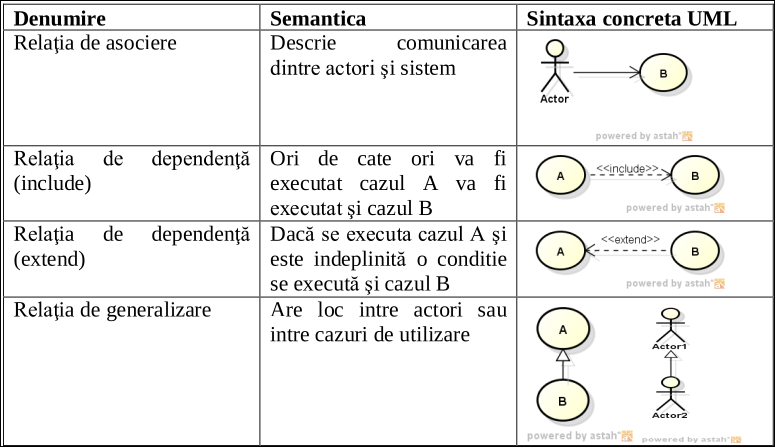
\includegraphics[width=0.9\textwidth]{assets/tipuri-relatii-uc.png}
\caption{Tipuri de relații în diagrama de cazuri de utilizare}
\label{fig:tipuri-relatii-uc}
\end{figure}

\newline

\begin{figure}[htbp]
\centering
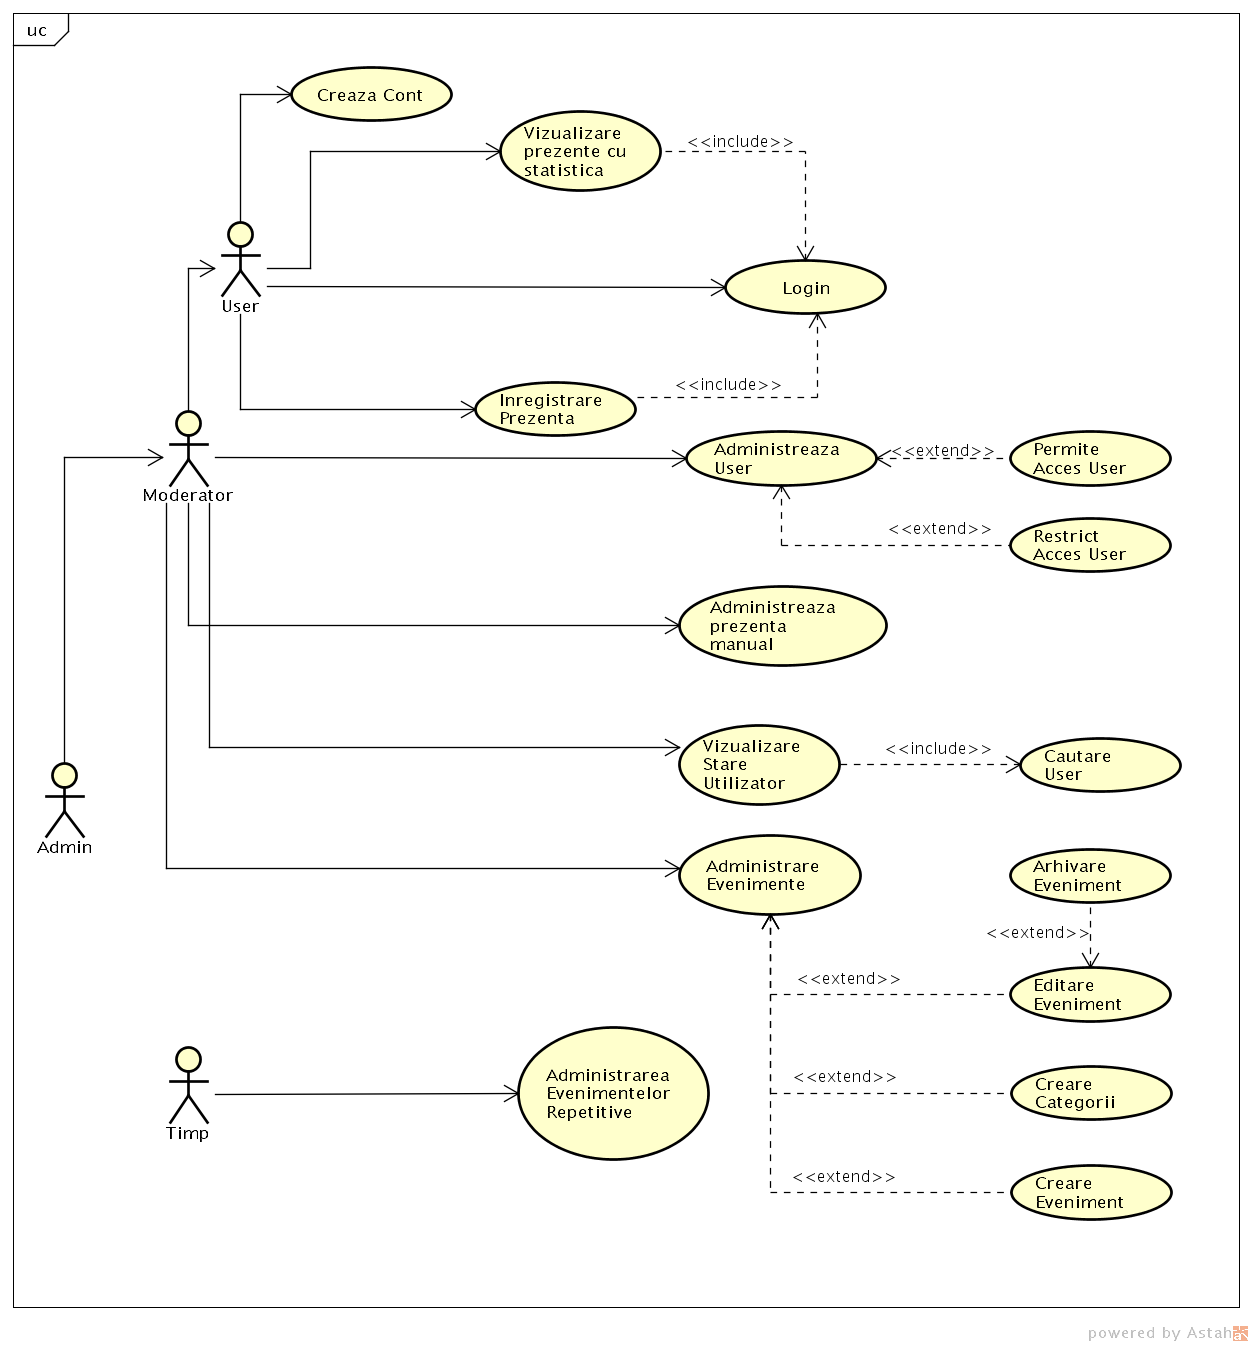
\includegraphics[width=0.9\textwidth]{assets/use-case-diagram.png}
\caption{Diagrama cazurilor de utilizare}
\label{fig:use-case-diagram}
\end{figure}

\section{Diagrame de secvențe de sistem}
\subsection{Evenimente de sistem}
Evenimentele de sistem apar datorită acțiunilor actorilor asupra sistemului software. Ele sunt de trei tipuri:
\begin{itemize}
    \item De flux de date (create de acțiuni ce transmit date sau informații)
    \item De control (nu conțin date)
    \item Temporare (evenimente generate de un cronjob)
\end{itemize}

După ce am analizat cazurile de utilizare am dedus următoarele evenimente de sistem:

\begin{table}[htbp]
\centering
\caption{Evenimente de sistem identificate}
\begin{tabular}{|l|l|p{0.5\textwidth}|}
\hline
\textbf{Tip} & \textbf{Nr.} & \textbf{Descriere} \\
\hline
Flux de date & 1 & Utilizatorul introduce datele de înregistrare sau logare și le trimite sistemului \\
\hline
Flux de date & 2 & Utilizatorul introduce codul primit pe adresa de mail electronică și îl trimite sistemului \\
\hline
Flux de date & 3 & Utilizatorul introduce numele unei categorii de eveniment în bara de căutare și trimite sistemului \\
\hline
Control & 4 & Sistemul marchează utilizatorul ca fiind prezent la evenimentul activ \\
\hline
Control & 5 & Sistemul autorizează accesul utilizatorului \\
\hline
Control & 6 & Sistemul verifică datele introduse de utilizator \\
\hline
Temporare & 7 & Sistemul creează evenimente în baza timpului setat de administrator \\
\hline
Temporare & 8 & Sistemul deschide prezența la evenimente dacă fereastra de prezență coincide cu timpul actual \\
\hline
\end{tabular}
\label{tab:evenimente-sistem}
\end{table}

\subsection{Diagrame de secvență de sistem}

Aceste diagrame descriu interacțiunea dintre actori și sistemul software. Interacțiunea e descrisă de mesaje, care la rândul lor reprezintă comunicarea dintre două obiecte.
Urmează să prezint conceptele diagramei de secvențe și a sintaxei în limbajul UML.
\newline

\begin{figure}[htbp]
\centering
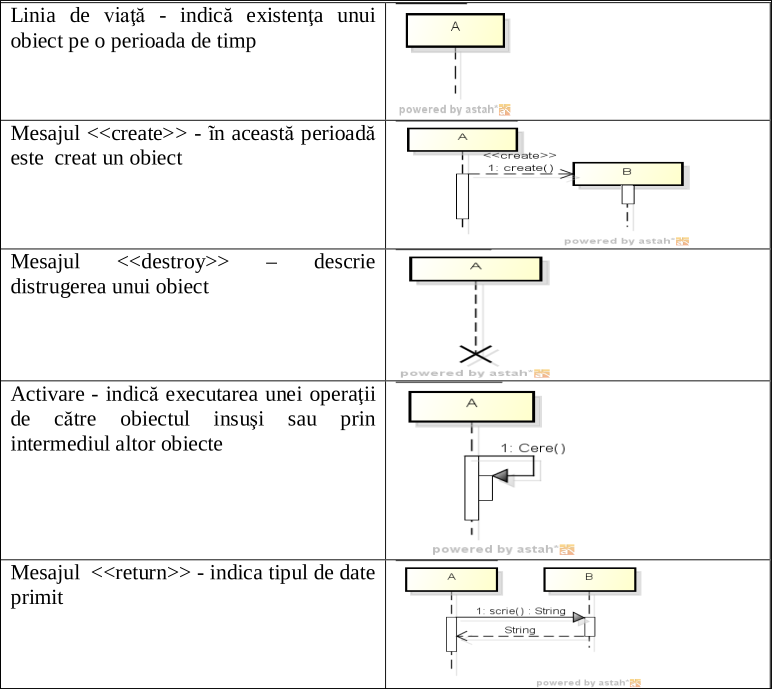
\includegraphics[width=0.85\textwidth]{assets/prezentare-diag-secvente.png}
\caption{Prezentarea diagramelor de secvență de sistem}
\label{fig:prezentare-diag-secvente}
\end{figure}

Așadar, acestea sunt diagramele de secvență de sistem pe care le-am făcut în urma analizei soluției mele.
\newline

\begin{figure}[htbp]
\centering
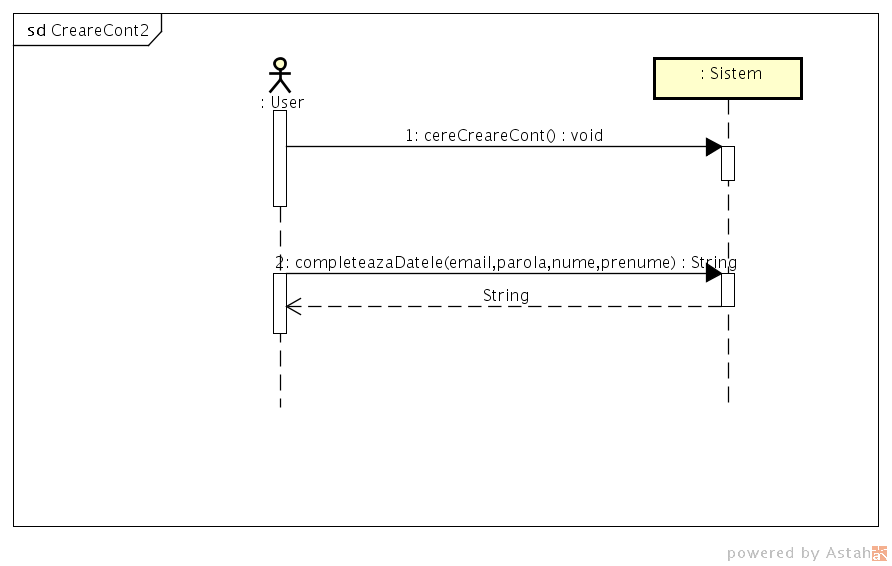
\includegraphics[width=0.9\textwidth]{assets/ssd-creare-cont.png}
\caption{Diagrama de secvență — Creare cont}
\label{fig:ssd-creare-cont}
\end{figure}

\begin{figure}[htbp]
\centering
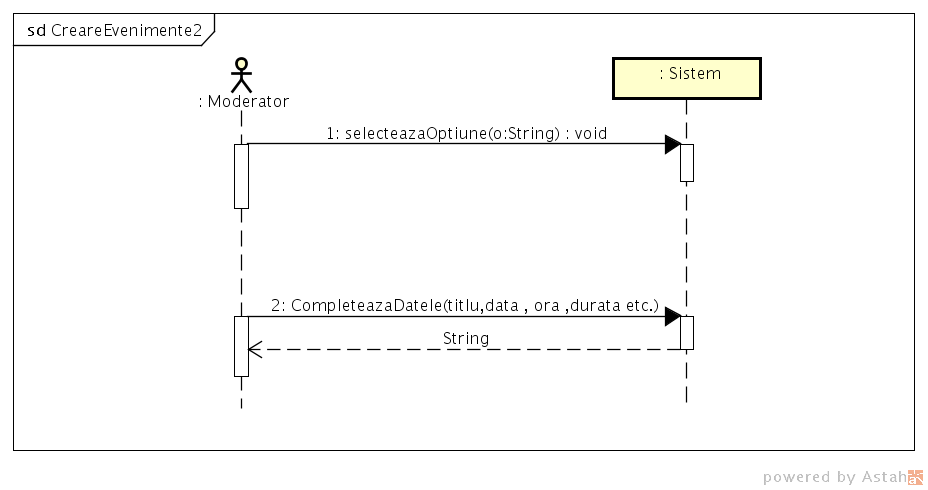
\includegraphics[width=0.9\textwidth]{assets/ssd-creare-evenimente.png}
\caption{Diagrama de secvență — Creare evenimente}
\label{fig:ssd-creare-evenimente}
\end{figure}

\begin{figure}[htbp]
\centering
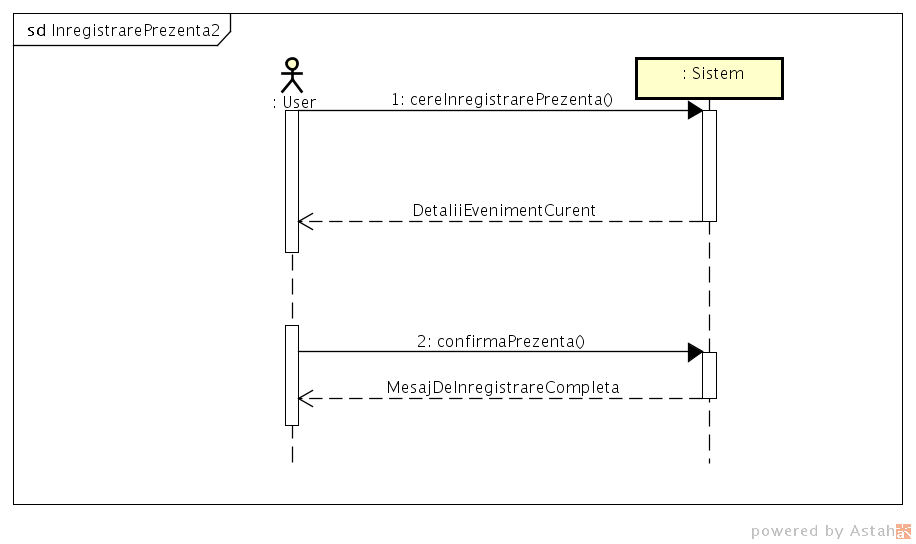
\includegraphics[width=0.9\textwidth]{assets/ssd-inregistrare-prezenta.png}
\caption{Diagrama de secvență — Înregistrare prezență}
\label{fig:ssd-inregistrare-prezenta}
\end{figure}

\begin{figure}[htbp]
\centering
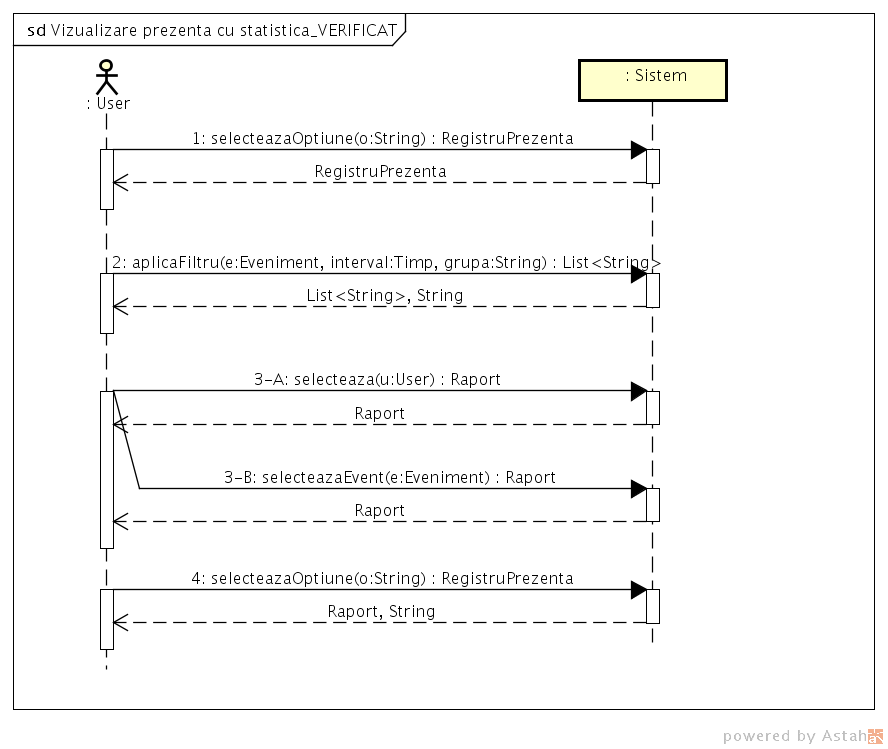
\includegraphics[width=0.9\textwidth]{assets/ssd-vizualizare-prezenta.png}
\caption{Diagrama de secvență — Vizualizare prezență}
\label{fig:ssd-vizualizare-prezenta}
\end{figure}



\bibliographystyle{unsrt}
\setlength{\baselineskip}{\normalbaselineskip}
\setlength{\parskip}{0pt}
\bibliography{refs}
\end{document}
